%%
%% This is file `sample-sigconf-authordraft.tex',
%% generated with the docstrip utility.
%%
%% The original source files were:
%%
%% samples.dtx  (with options: `all,proceedings,bibtex,authordraft')
%% 
%% IMPORTANT NOTICE:
%% 
%% For the copyright see the source file.
%% 
%% Any modified versions of this file must be renamed
%% with new filenames distinct from sample-sigconf-authordraft.tex.
%% 
%% For distribution of the original source see the terms
%% for copying and modification in the file samples.dtx.
%% 
%% This generated file may be distributed as long as the
%% original source files, as listed above, are part of the
%% same distribution. (The sources need not necessarily be
%% in the same archive or directory.)
%%
%%
%% Commands for TeXCount
%TC:macro \cite [option:text,text]
%TC:macro \citep [option:text,text]
%TC:macro \citet [option:text,text]
%TC:envir table 0 1
%TC:envir table* 0 1
%TC:envir tabular [ignore] word
%TC:envir displaymath 0 word
%TC:envir math 0 word
%TC:envir comment 0 0
%%
%% The first command in your LaTeX source must be the \documentclass
%% command.
%%
%% For submission and review of your manuscript please change the
%% command to \documentclass[manuscript, screen, review]{acmart}.
%%
%% When submitting camera ready or to TAPS, please change the command
%% to \documentclass[sigconf]{acmart} or whichever template is required
%% for your publication.
%%
%%
\documentclass[review,anonymous,acmtog]{acmart}
\acmSubmissionID{tcom\_122}
%%
%% \BibTeX command to typeset BibTeX logo in the docs
\AtBeginDocument{%
  \providecommand\BibTeX{{%
    Bib\TeX}}}

\usepackage{amsmath}
\usepackage{setspace}
\usepackage{titlesec}
\usepackage[percent]{overpic}
\usepackage{lipsum}  

\newcommand{\TODO}[2]{{\color{blue} {#1}}}
\graphicspath{{figures/}{pictures/}{images/}{./}} % where to search for the images

%% We encourage the use of mathptmx for consistent usage of times font
%% throughout the proceedings. However, if you encounter conflicts
%% with other math-related packages, you may want to disable it.
\usepackage{mathptmx}                  % use matching math font
\usepackage{adjustbox} 
\usepackage{placeins}

\usepackage{graphicx}  % For including images
\usepackage{stfloats}  % Helps keep floats at the top
\usepackage{caption}   % Allows fine-tuned caption spacing

\usepackage{xcolor}

\usepackage{float} 
\usepackage{wrapfig}
\usepackage{lipsum}

%% Rights management information.  This information is sent to you
%% when you complete the rights form.  These commands have SAMPLE
%% values in them; it is your responsibility as an author to replace
%% the commands and values with those provided to you when you
%% complete the rights form.
% \setcopyright{acmlicensed}
% \copyrightyear{2018}
% \acmYear{2018}
% \acmDOI{XXXXXXX.XXXXXXX}
%% These commands are for a PROCEEDINGS abstract or paper.
% \acmConference[Conference acronym 'XX]{Make sure to enter the correct
%   conference title from your rights confirmation email}{June 03--05,
%   2018}{Woodstock, NY}
%%
%%  Uncomment \acmBooktitle if the title of the proceedings is different
%%  from ``Proceedings of ...''!
%%
%%\acmBooktitle{Woodstock '18: ACM Symposium on Neural Gaze Detection,
%%  June 03--05, 2018, Woodstock, NY}
% \acmISBN{978-1-4503-XXXX-X/2018/06}


%%
%% Submission ID.
%% Use this when submitting an article to a sponsored event. You'll
%% receive a unique submission ID from the organizers
%% of the event, and this ID should be used as the parameter to this command.
%%\acmSubmissionID{123-A56-BU3}

%%
%% For managing citations, it is recommended to use bibliography
%% files in BibTeX format.
%%
%% You can then either use BibTeX with the ACM-Reference-Format style,
%% or BibLaTeX with the acmnumeric or acmauthoryear sytles, that include
%% support for advanced citation of software artefact from the
%% biblatex-software package, also separately available on CTAN.
%%
%% Look at the sample-*-biblatex.tex files for templates showcasing
%% the biblatex styles.
%%

%%
%% The majority of ACM publications use numbered citations and
%% references.  The command \citestyle{authoryear} switches to the
%% "author year" style.
%%
%% If you are preparing content for an event
%% sponsored by ACM SIGGRAPH, you must use the "author year" style of
%% citations and references.
%% Uncommenting
%% the next command will enable that style.
\citestyle{acmauthoryear}


%%
%% end of the preamble, start of the body of the document source.
\begin{document}

%%
%% The "title" command has an optional parameter,
%% allowing the author to define a "short title" to be used in page headers.
\title{New Methods for Mesh Intersection Repair}

%%
%% The "author" command and its associated commands are used to define
%% the authors and their affiliations.
%% Of note is the shared affiliation of the first two authors, and the
%% "authornote" and "authornotemark" commands
%% used to denote shared contribution to the research.

\author{Kenichi Maeda}
\affiliation{%
  \institution{University of Massachusetts Boston}
  \city{Boston}
  \country{USA}}
\email{kenichi.maeda001@umb.edu}

\author{Daniel Haehn}
\authornote{Joint senior author}
\affiliation{%
  \institution{University of Massachusetts Boston}
  \city{Boston}
  \country{USA}}
\email{daniel.haehn@umb.edu}

\author{Sumientra Rampersad}
\authornote{Joint senior author}
\affiliation{%
  \institution{University of Massachusetts Boston}
  \city{Boston}
  \country{USA}}
\email{sumientra.rampersad@umb.edu}

%%
%% By default, the full list of authors will be used in the page
%% headers. Often, this list is too long, and will overlap
%% other information printed in the page headers. This command allows
%% the author to define a more concise list
%% of authors' names for this purpose.
\renewcommand{\shortauthors}{Trovato et al.}

%%
%% The abstract is a short summary of the work to be presented in the
%% article.
\begin{abstract}
  Triangular surface meshes have many uses in science and engineering. A common problem in mesh geometry is having intersections of multiple facets within one mesh, or between two meshes. This issue has been addressed for decades, resulting in many repair algorithms and tools, whether open source or commercial. Although all these methods achieve the purpose of repairing intersections, their performance varies from one another due to differences in approach and implementation. In our studies, we evaluate how different tools and algorithms affect the repair outcomes both visually and quantitatively, using a comprehensive set of mesh quality metrics. Moreover, even high-quality repairs might not be optimal depending on the specific use case of the mesh. Our goal is to assess not only how well the mesh has been repaired, but also to what extent the repair has structurally changed the geometry. Finally, we introduce a new repair method that is efficient and does not affect the integrity of the mesh. Furthermore, we look at two situations in which intersections require a different approach from the ones currently available, and propose potential strategies for addressing them.
\end{abstract}

%%
%% The code below is generated by the tool at http://dl.acm.org/ccs.cfm.
%% Please copy and paste the code instead of the example below.
%%
% \begin{CCSXML}
% <ccs2012>
%  <concept>
%   <concept_id>00000000.0000000.0000000</concept_id>
%   <concept_desc>Do Not Use This Code, Generate the Correct Terms for Your Paper</concept_desc>
%   <concept_significance>500</concept_significance>
%  </concept>
%  <concept>
%   <concept_id>00000000.00000000.00000000</concept_id>
%   <concept_desc>Do Not Use This Code, Generate the Correct Terms for Your Paper</concept_desc>
%   <concept_significance>300</concept_significance>
%  </concept>
%  <concept>
%   <concept_id>00000000.00000000.00000000</concept_id>
%   <concept_desc>Do Not Use This Code, Generate the Correct Terms for Your Paper</concept_desc>
%   <concept_significance>100</concept_significance>
%  </concept>
%  <concept>
%   <concept_id>00000000.00000000.00000000</concept_id>
%   <concept_desc>Do Not Use This Code, Generate the Correct Terms for Your Paper</concept_desc>
%   <concept_significance>100</concept_significance>
%  </concept>
% </ccs2012>
% \end{CCSXML}

% \ccsdesc[500]{Computing methodologies~Generate the Correct Terms for Your Paper}
% \ccsdesc[300]{Do Not Use This Code~Generate the Correct Terms for Your Paper}
% \ccsdesc{Do Not Use This Code~Generate the Correct Terms for Your Paper}
% \ccsdesc[100]{Do Not Use This Code~Generate the Correct Terms for Your Paper}

\begin{CCSXML}
<ccs2012>
   <concept>
    <concept_id>10003120.10003145.10011769</concept_id>
       <concept_desc>Human-centered computing~Empirical studies in visualization</concept_desc>
       <concept_significance>300</concept_significance>
       </concept>
   <concept>
       <concept_id>10010147.10010371.10010396.10010397</concept_id>
       <concept_desc>Computing methodologies~Mesh models</concept_desc>
       <concept_significance>500</concept_significance>
       </concept>
 </ccs2012>
\end{CCSXML}

\ccsdesc[300]{Computing methodologies~Modeling methodologies}
\ccsdesc[300]{Human-centered computing~Empirical studies in visualization}
\ccsdesc[500]{Computing methodologies~Mesh models}

%%
%% Keywords. The author(s) should pick words that accurately describe
%% the work being presented. Separate the keywords with commas.
\keywords{finite element model, triangular surface mesh, self-intersection, intersection, mesh repair}
%% A "teaser" image appears between the author and affiliation
%% information and the body of the document, and typically spans the
%% page.
\begin{teaserfigure}
  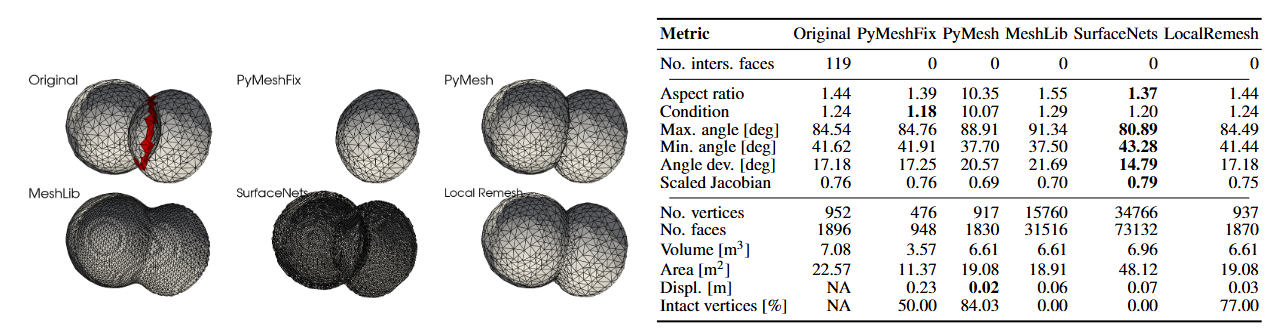
\includegraphics[width=\textwidth]{figures/teaser_3.png}
  \caption{\textbf{Merging two neighboring meshes.} Visual (left) and quantitative (right) comparison of mesh quality for the original and repaired meshes in test case 1 using five different repair methods. Figures show the inside of each mesh with intersections marked in red. In the tables, all metrics from aspect ratio to intact vertices are the mean value across the entire output mesh. For each metric, the value of the best-performing mesh is shown in bold.}
  \label{fig:teaser}
\end{teaserfigure}


% \received{20 February 2007}
% \received[revised]{12 March 2009}
% \received[accepted]{5 June 2009}

%%
%% This command processes the author and affiliation and title
%% information and builds the first part of the formatted document.
\maketitle

\section{Introduction}
Today, 3D triangular surface meshes are used for a wide variety of purposes. Due to their ability to model objects efficiently, accurately, and in a customizable manner, they are commonly utilized in modeling, manufacturing, computer graphics, and geometry-based simulations. A mesh is often modeled from a real-world object, and hence it is not uncommon to see defects. Ju defines \textit{geometric correctness} as a state in which a mesh is watertight and free from defects \cite {ju2009geometric_errors}. Mesh defects are geometric errors, which include, but are not limited to, gaps, holes, non-manifold elements, and self-intersections. 

In this study, we specifically investigate intersections, a common defect where multiple components (i.e., facets or edges) within one mesh, or between two meshes, intersect each other. This may occur when surface meshes are created from image segmentations in which some of the compartments are locally thinner than a single voxel. Such intersecting surfaces do not allow the construction of a volume mesh, which is required for finite element modeling (FEM), a common mesh-based simulation method.

To address this issue, tools have been developed that can fix intersections. While some methods produce geometrically correct meshes, they may delete crucial mesh components, or introduce new problems such as low-quality elements. There is a need to find an optimal method depending on how much modification and complexity we allow, considering the intended application of the repaired mesh. Therefore, in this study, we consider not only geometric correctness of the repaired meshes, but also the quality of their triangles, and their structural integrity with respect to the input meshes. 

\subsection{Related Work}
When reviewing past work on intersection repairs, one can see two main approaches. The first involves removing intersecting components, whether they are facets or edges, and then patching the resulting holes. This is considered the simplest, most intuitive, and computationally lightweight method. Attene introduced such an algorithm to convert a mesh with defects into a single watertight triangular mesh~\cite{attene2010lightweight}. The algorithm iteratively eliminates intersecting triangles and their neighbors, then patches the resulting gaps with new edges and facets, until no self-intersections are detected. The main issue with this algorithm is that disconnected components may be removed during the degeneracy removal process. 

Another common approach is to detect intersections and resolve them by adding extra edges and vertices along crossing lines for triangulations. Its main advantage is that it does not involve major deletion and preserves the original mesh as much as possible; thus significant changes in volume and shape are not expected. Zhu developed an algorithm following this principle~\cite{Zhu2019robustalgo}. In his “direct repair algorithm,” Attene achieved the same goal by subdividing triangles along their intersecting elements~\cite{attene2014directrepair}. Although there are some variations of this approach, they all perform reasonably well in terms of retaining the original mesh structure~\cite{cherchi2020floating, charton2021topology}. However, this method is likely to create narrow and skewed triangles near areas where intersections once existed. If the sole objective is to remove intersections, this may not be a significant concern. However, in cases where mesh quality is crucial, such as in FEM, this can be problematic, as poorly shaped elements can negatively affect stability, accuracy, and convergence of the simulation~\cite{nemade2020meshquality}.

While the approaches discussed so far are considered mesh-based (or surface-based) repair methods, one can also voxelize a mesh (i.e., create a 3D cubic grid that resembles the shape of the surface mesh) and then create a completely new mesh based on this voxel grid~\cite{ju2009geometric_errors, sfikas2022FoR}, known as voxel-based repair. Several well-known algorithms, such as marching cubes \cite{Lorensen1987marchingcubes}, can be used to create the desired mesh~\cite{ju2009geometric_errors, sfikas2022FoR}. After this modification, no defects should remain \cite{sfikas2022FoR}. However, this method also presents challenges related to mesh quality, largely determined by the voxel size. If the voxel size is too large, the mesh loses a significant amount of its original information. If it is too small, the mesh complexity increases dramatically, resulting in a substantial computational burden for simulations.

Our goal in this study is to evaluate existing mesh repair approaches and assess their performance in terms of geometric correctness (i.e., amount of defects), mesh quality (i.e., triangle shape), and structural integrity (i.e., preservation of geometric features). 
We consider a wide range of quality metrics and evaluate their merits for this purpose. Furthermore, we explore alternative methods for resolving intersections, such as local remeshing and detaching sub-meshes, and examine their suitability for different scenarios. We provide all implemented algorithms, evaluation metrics, visualization methods, and data through our GitHub page.

\section{General approach}

We will examine three different variations of mesh intersections. To illustrate these situations, we will consider a finite element model of a human head. Such models contain a triangular surface mesh for each tissue boundary, e.g., skull and brain, based on the segmentation of an MRI scan. The human brain presents a modeling challenge since its outer surface consists of ridges called gyri that are closer together than the width of a single MRI voxel. If two neighboring gyri intersect, we can choose to either merge or detach the two gyri, depending on the application. A different situation that causes intersections is when two enclosed meshes intersect with each other, for example, in areas where the brain and skull touch. In this study, we represent these cases with simple geometries that are easier to visualize and quantify. For example, we used two individual spheres that intersect on one side to represent two gyri on one surface intersecting (Fig. \ref{fig:teaser}, first image), and two enclosed spheres to represent a brain and skull surface intersecting (Fig. \ref{fig:sol2-2}, left). These simple geometries closely represent the local problems encountered in large complex structures. For example, a brain surface may have many self-intersecting gyri, each of which resembles the case of two spheres, and can be repaired in the same way. To ensure a comprehensive comparison, test meshes of varying complexity were generated using Blender. We created three test cases with two neighboring meshes and one with two enclosed meshes.

In all cases, we aimed to achieve three goals: 1) fix all intersections without producing other defects such as holes, 2) produce a high-quality mesh, and 3) preserve the original shape and position of the mesh as much as possible. To accomplish this, we can either locally resolve intersecting areas, or we can globally remesh the model. We applied and compared five different methods to merge two neighboring meshes. This approach is sufficient for most cases and is commonly adopted in existing repair functions across various mesh libraries. We also developed one method to detach two neighboring meshes and one method to detach two enclosed meshes. Ideally, the final output in each case should have no intersections and no significant shape alterations. 

To quantitatively assess the output meshes, we  evaluated them using the mesh metrics and statistics shown in Table 1 in the supplemental material. In this study, we place greater emphasis on mesh quality than on computational efficiency, as we evaluate the final mesh condition. Ideally, a high-quality triangular mesh consists of elements that are as close to equilateral as possible. Each metric was evaluated based on this assumption. Metrics marked with an asterisk were computed using PyVista, a wrapper of VTK. The rest were calculated manually. Each test mesh contains noise, in the form of self-intersections. These evaluations were performed on a computer with an 11th Gen Intel Core CPU and 12.0 GB of RAM. 

% \begin{figure*}[t]
%   \centering
%   \begin{minipage}{0.45\textwidth}
%     \centering
%     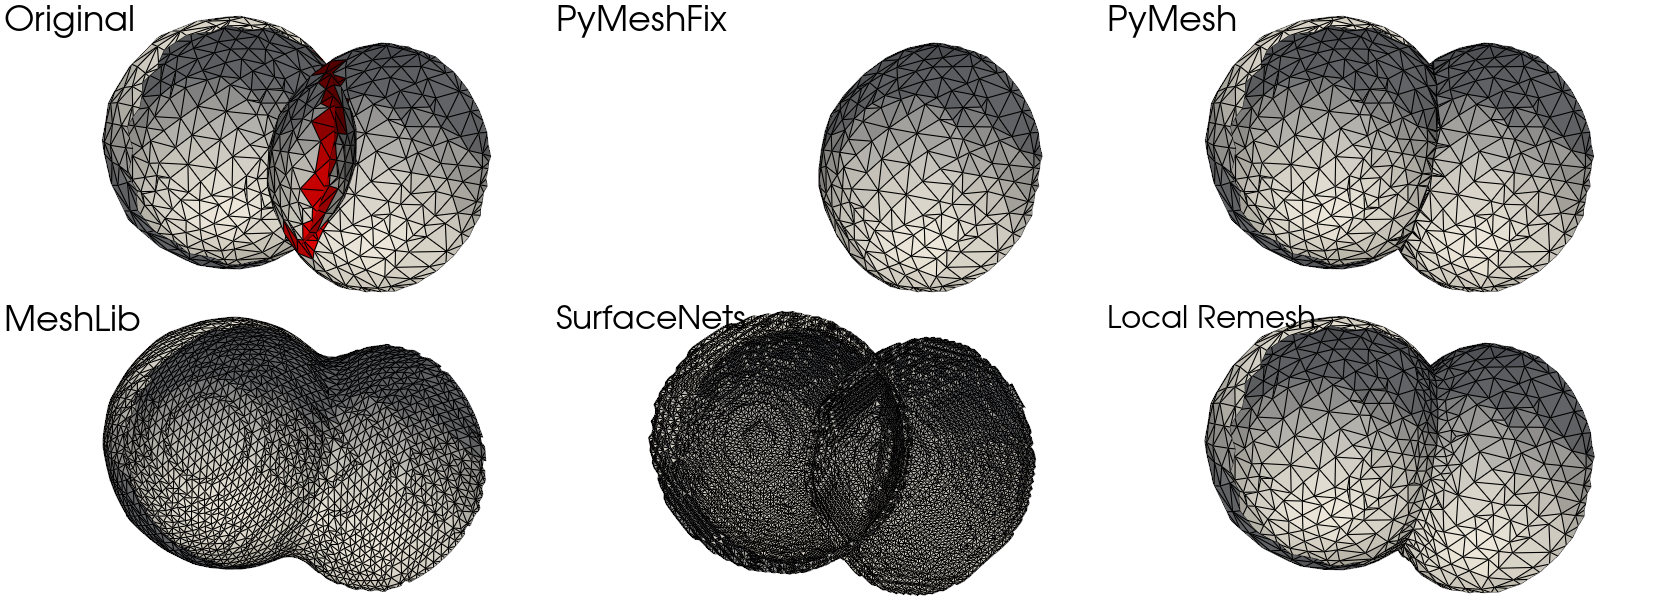
\includegraphics[width=\linewidth]{../figures/test_case1_inner.png}
%     % 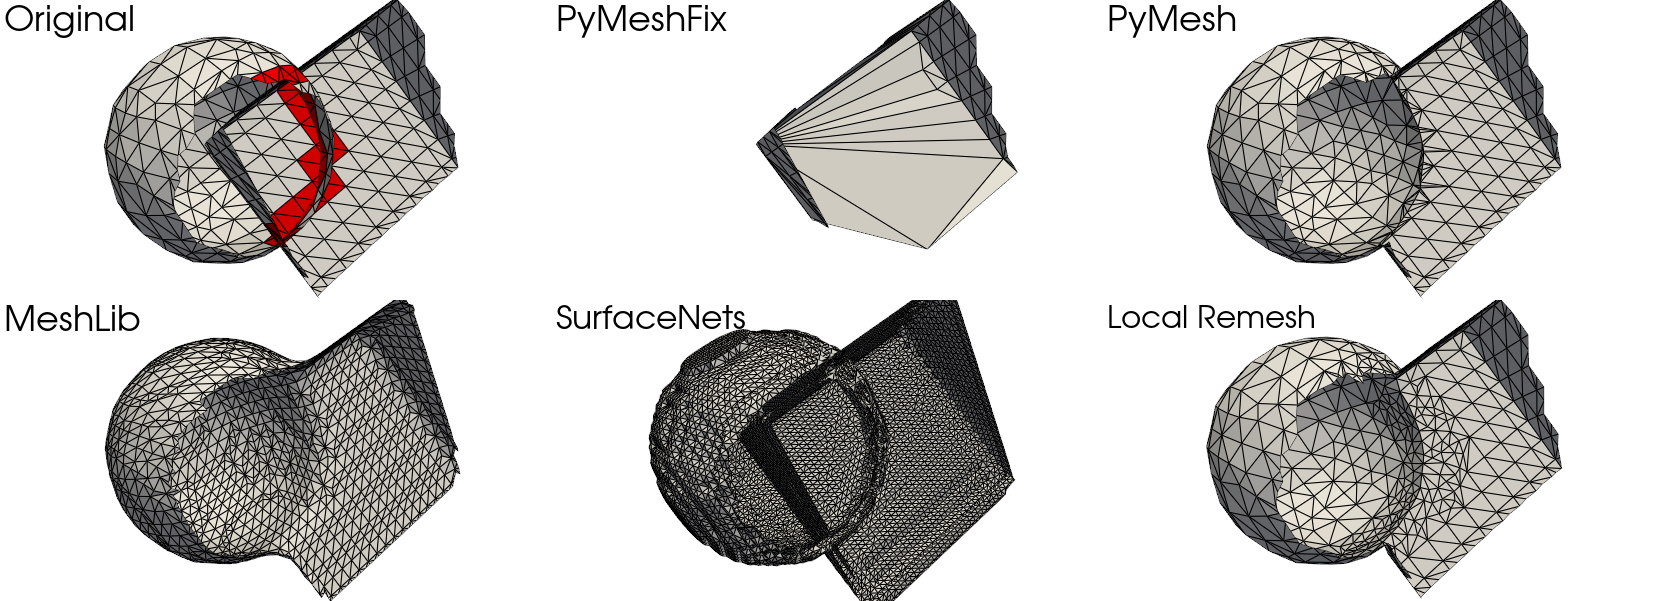
\includegraphics[width=\linewidth]{../figures/test_case3_inner.png}
%   \end{minipage}
%   \begin{minipage}{0.54\textwidth}
%     \centering
%     \renewcommand{\arraystretch}{0.45}
%     \small
%     \setlength{\tabcolsep}{1.2pt}
%     \begin{tabular}{lrrrrrr}
%         \toprule
%         \textbf{Metric} & Original & PyMeshFix & PyMesh & MeshLib & SurfaceNets & LocalRemesh \\
%         \midrule
%         No. vertices                & 952       & 476       & 917       & 15760      & 34766 & 937       \\
%         No. faces                   & 1896      & 948       & 1830      & 31516     & 73132 & 1870      \\
%         No. inters. faces  & 119       & 0         & 0         & 0        &  0  & 0         \\
%         Volume [m$^3$]                 & 7.08     & 3.57     & 6.61     & 6.61  & 6.96 & 6.61     \\
%         Area [m$^2$]                    & 22.57    & 11.37    & 19.08    & 18.91   & 48.12 & 19.08    \\
%         Aspect ratio       & 1.44     & 1.39     & 10.35    & 1.55    & \textbf{1.37}  & 1.44  \\
%         Condition          & 1.24     & \textbf{1.18}     & 10.07    & 1.29 & 1.20 & 1.24  \\
%         Max. angle [deg]          & 84.54    & 84.76    & 88.91    & 91.34 & \textbf{80.89}& 84.49  \\
%         Min. angle [deg]          & 41.62    & 41.91    & 37.70    & 37.50& \textbf{43.28}& 41.44  \\
%         Angle dev. [deg]    & 17.18    & 17.25    & 20.57    & 21.69& \textbf{14.79}& 17.18     \\
%         Scaled Jacobian    & 0.76     & 0.76     & 0.69     & 0.70& \textbf{0.79}& 0.75  \\
%         Displ. [m]      & NA       & 0.23     & \textbf{0.02} & 0.06  & 0.07& 0.03  \\
%         Intact vertices [\%]    & NA       & 50.00        & 84.03    & 0.00         & 0.00    & 77.00     \\
%         \bottomrule
%     \end{tabular}\par\vspace{5mm}

%     % \iffalse
%     % \begin{tabular}{lrrrrrr}
%     %     \toprule
%     %     \textbf{Metric} & Original & PyMeshFix & PyMesh & MeshLib & SurfaceNets & LocalRemesh \\
%     %     \midrule
%     %     No. vertices                & 1608      & 536       & 1576      & 26588& 61786 & 1564      \\
%     %     No. faces                   & 3204      & 1068      & 3148      & 53172& 129624 & 3124      \\
%     %     No. inters. face pairs  & 292       & 0         & 0         & 0        & 0     & 0         \\
%     %     Volume [m$^3$]                  & 11.96    & 3.99     & 11.02    & 11.02 & 11.60 & 11.01    \\
%     %     Area [m$^2$]                    & 36.60    & 12.20    & 29.38    & 29.08& 78.29 & 29.38    \\
%     %     Mean aspect ratio       & 1.33     & \textbf{1.33}     & 7.59   & 1.56& 1.41 & 1.37  \\
%     %     Mean condition          & 1.15     & \textbf{1.15}     & 7.33   & 1.30 & 1.24 & 1.18  \\
%     %     Mean max angle  [deg]         & 81.72    & 81.72    & 88.20    & 91.43 & \textbf{80.21}& 82.75  \\
%     %     Mean min angle  [deg]         & 41.22    & 41.22    & 36.63    & 37.58& \textbf{43.67}& 41.01  \\
%     %     Mean scaled Jacobian    & 0.76     & 0.76     & 0.67     & 0.70     & \textbf{0.79}& 0.75  \\
%     %     Mean displ. [m]       & NA       & 0.36     & \textbf{0.03}  & 0.06& 0.07& 0.04  \\
%     %     Mean angle dev. [deg]    & 15.73    & 15.73    & 20.16    & 21.80 & \textbf{14.35}& 16.37     \\
%     %     Intact vertices [\%]    & NA       & 33.33    & 80.35    & 0.00& 0.00& 70.65     \\
%     %     \bottomrule
%     % \end{tabular}\par\vspace{2mm}
%     % \fi

%     % \begin{tabular}{lrrrrrr}
%     %     \toprule
%     %     \textbf{Metric} & Original & PyMeshFix & PyMesh & MeshLib & SurfaceNets & LocalRemesh \\
%     %     \midrule
%     %     No. vertices                & 760       & 230       & 758       & 11064& 23773 & 860       \\
%     %     No. faces                   & 1512      & 456       & 1512      & 22124& 48932 & 1716      \\
%     %     No. inters. faces  & 99        & 0         & 0         & 0& 0 & 0         \\
%     %     Volume [m$^3$]                  & 11.59    & 6.95     & 10.85    & 10.817& 5.43& 10.84    \\
%     %     Area [m$^2$]                    & 34.64    & 25.12    & 29.92    & 29.30& 69.64 & 29.92    \\
%     %     Aspect ratio       & 1.39     & 2.21     & 2.13     & 1.52 & \textbf{1.40} & 1.42  \\
%     %     Condition          & 1.18     & 1.87     & 1.86     & 1.27 & \textbf{1.18} & 1.20  \\
%     %     Max. angle [deg]          & 86.46    & 96.10    & 90.45    & 90.82& \textbf{85.88}& 86.31  \\
%     %     Min. angle [deg]          & 41.66    & 35.01    & 38.04    & 37.51& \textbf{41.32}& 40.87  \\
%     %     Angle dev. [deg]    & 17.91    & 24.37    & 20.88    & 21.07& \textbf{17.65}& 18.07     \\
%     %     Scaled Jacobian    & 0.76     & 0.65     & 0.70     & 0.70 & \textbf{0.76}& 0.75  \\
%     %     Displ. [m]       & NA       & 0.31     & \textbf{0.03}     & 0.08& 0.11 & 0.04  \\
%     %     Intact vertices [\%]    & NA       & 30.26    & 86.71    & 0.00& 0.00& 79.74     \\
%     %     \bottomrule
%     % \end{tabular}
%   \end{minipage}
%   \caption{\textbf{Merging two neighboring meshes.} Visual (left) and quantitative (right) comparison of mesh quality for the original and repaired meshes in test case 1 (top) and 2 (bottom) using five different repair methods. Figures show the inside of each mesh with intersections marked in red. In the tables, all metrics from aspect ratio to angle deviation are the mean value across the entire output mesh. For each metric, the value of the best-performing mesh is shown in bold.}
%   \label{fig:wide_combo}
% \end{figure*}

\section{Merging neighboring meshes}
We selected the five methods described below based on their usability, high performance, popularity, and the uniqueness of their functionalities.
\textbf{PyMeshFix}: A mesh-based repair. It first removes self-intersecting triangles and then fills the resulting holes. We called the function \texttt{pymeshfix.clean\_from\_arrays()} from PyMeshFix, a Python wrapper for MeshFix, developed by Attene \cite{attene2010lightweight}.
\textbf{PyMesh}: A mesh-based repair. It fixes self-intersections by subdividing intersecting facets, adding new vertices and edges as needed. We called the fuction \texttt{pymesh.compute\_outer\allowbreak\_hull()} from PyMesh, which internally calls a function to resolve self-intersections during execution. The libgil engine runs in the background of this function call \cite{jacobson2018libigl}.  \textbf{MeshLib}: A voxel-based repair. MeshLib is an open-source 3D mesh library designed for geometry processing. We called \texttt{mrmeshpy.fixSelf\allowbreak Intersections()} for self-intersection resolution. For voxelization, the voxel size was set to a quarter of the median edge length. 
\textbf{SurfaceNets}: A voxel-based repair. In her study, Frisken extended 3D SurfaceNets to generate high-resolution and smooth 3D meshes from multi-labeled segmented volumes \cite{frisken2022surfacenets}. It enables the generation of a mesh with sharp boundaries preserved from the input after applying surfacing methods. In this evaluation, we used the original C++ implementation. The voxel size was set to a quarter of the median edge length here as well. 
\textbf{LocalRemesh}: A mesh-based repair. We implemented a method that locally remeshes intersecting areas. As mentioned earlier, a common challenge faced by many mesh-based repair methods that involve subdividing facets is the generation of ill-shaped triangles in the output mesh, which negatively impacts mesh quality. To address this, this method ensures that even after subdivision, any ill-shaped triangles are corrected through local remeshing. This was implemented using existing mesh libraries including trimesh. 


Test Case 1 consists of two intersecting spheres. The left side of Figure \ref{fig:teaser} shows the original state and the state after repair for all five methods. 
The various methods can be seen to produce structurally different results. However, all resulted in no intersections, indicating that each method achieved geometric correctness. 

When looking at our mesh quality metrics, SurfaceNets produced a mesh with better overall mesh quality, indicating that the repaired mesh has well-shaped triangles on its surface. The evaluation results also highlight strong performance of Meshlib. This can be attributed to the fact that both SurfaceNets and MeshLib repair self-intersections through global remeshing. The mesh gets a new surface during the process, which results in high-quality triangles. However, it is important to note that the performance of global remeshing methods depends on the voxel size. In this evaluation, the voxel size was set to a quarter of the median edge length. If we had chosen the voxel size to be larger or smaller, the performance could have been better or worse, changing how these methods compare to the others. 

In reviewing structural integrity, some methods successfully preserved the original geometry, while others did not.  PyMeshFix produced a mesh with one of the components missing after the repair, because the algorithm only keeps the largest component of the mesh and discards the rest. This would not be an issue with a self-intersecting mesh such as a brain that has intersecting gyri. However, in cases where intersections are due to submeshes, such as the two components shown here, the output would greatly deviate from the original geometry. PyMesh and SurfaceNets produced output meshes that have inner boundaries between the original components, with SurfaceNets leaving the original boundaries unchanged and PyMesh merging the two intersecting sections into one. These options may or may not be a viable solution depending on the application. For example, a volume mesh algorithm that fills triangular meshes with tetrahedral elements may not be able to process such a mesh. MeshLib and LocalRemesh created meshes without inner components, such that the resulting mesh forms an outer hull of the original mesh. For the purpose of creating a finite element volume mesh, such solutions are ideal.

In terms of geometric correctness and structural integrity, the repair algorithm of PyMesh can be considered stable. However, when we focus on mesh quality, the repaired meshes raise concerns for practical applications. Figure \ref{fig:sol1-analysis} shows a closer look at the repaired mesh from Test Case 1. As can be seen in the figure, the repaired sections consist of ill-shaped triangles. In such a geometry, both large and small angles could have detrimental effects on finite element modeling. The LocalRemesh method is based on PyMesh, but performs additional local remeshing to eliminate the ill-shaped triangles produced by PyMesh. These differences are reflected in the calculated metrics as PyMesh having 1) smaller differences between the original and output mesh (smaller displacement and higher percentage of intact vertices), and 2) worse results in all triangle quality metrics (maximum and minimum angle, angle deviation, aspect ratio, condition and scaled Jacobian). This example demonstrates the importance of carefully evaluating quality metrics, and choosing a mesh repair method based on metrics that reflect the desired output.

Further test cases are presented in the supplemental material. % and the meshes can be viewed interactively online.
The produced results are structurally similar to what we saw for Test Case 1. In addition to basic geometric shapes, we also assessed these methods with a brain surface mesh created from a T1-weighted MRI scan of a 28-year-old male. Figure 1 in the supplemental material shows the results. For complicated cases like this, there is a need to be more careful, as the resulting differences are less visually obvious compared to simple ones.


\begin{figure}[h]
    \centering
    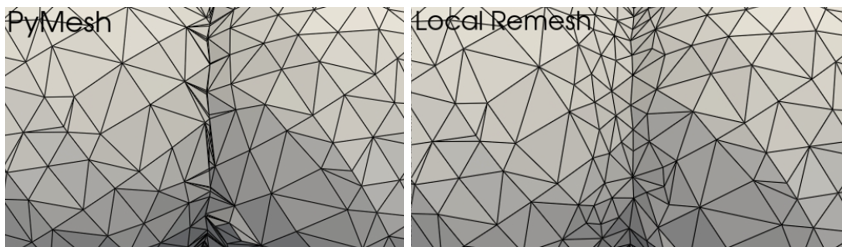
\includegraphics[width=0.90\linewidth, height=2.4cm]{../figures/3.png}
     \caption{\textbf{Closeup of LocalRemesh vs PyMesh.} Both methods repaired the intersections between two neighboring meshes, but LocalRemesh produced a result of much higher quality.}
     \label{fig:sol1-analysis}
\end{figure}
\section {Detaching neighboring meshes}
Alternatively, instead of merging neighboring intersecting meshes, we can also remove intersections by cutting the mesh into individual components. This approach is required for specific applications. For example, when using FEM to solve an equation that describes a physics problem, each component needs to be assigned its own physical properties (e.g., electric conductivity) and thus its boundaries need to be clearly defined. A different example is the brain model described before, in which the individual gyri of one mesh may intersect. While they are not physically separate organs, each gyrus is an anatomical entity with its own function. Hence, an individual, intersection-free mesh representation of each gyrus might be needed, for example, in high resolution FEM. In addition, the local directions of neurons are defined as perpendicular to the surface, so directions remain unknown in areas without a surface. We did not find any methods that solve this problem. Here we present our implementation. It first cuts an intersecting mesh into submeshes by removing self-intersecting facets. That removal may introduce holes and small floating components. Next, the method retains only the primary submeshes of interest, and discards the rest. The resulting holes are then patched. While this method does not preserve the original geometry, its main goal is to differentiate submeshes that are meant to represent different entities. Figure \ref{fig:sol3-2} shows the original and repaired mesh for Test Case 1. Our method produced
geometrically correct meshes of reasonable quality. Another test case is presented in the supplemental material. We aim to further improve this method to produce higher quality results.

\vspace{-0.5em}

\begin{figure}[h]
    \centering
    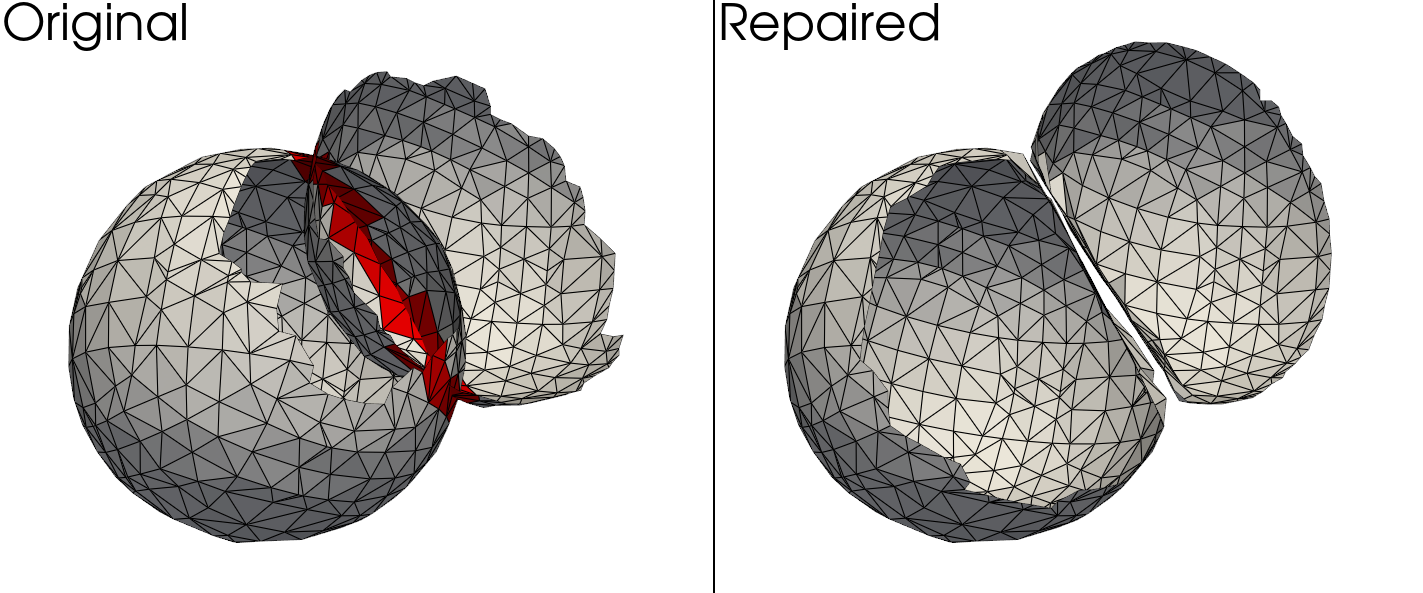
\includegraphics[width=0.6\linewidth, height=2.2cm]{../figures/detach_n_1.png}
    \caption{\textbf{Detaching neighboring meshes.} Original and repaired mesh for test case 1. The meshes have been divided into two distinct pieces, as opposed to the solution shown in Fig. \ref{fig:sol2-2}.}
    \label{fig:sol3-2}
\end{figure}

\vspace{-1em}
\section{Detaching enclosed meshes}
In biomedical problems, volume meshes are often constructed from multiple surfaces enclosed in another, where each surface represents an organ or piece of tissue. Due to their complicated shape and close proximity, it is common to obtain intersections between these surfaces. Even when each segmented mesh is individually free of self-intersections, additional intersections can arise when they are merged into a single mesh. This makes producing a volume mesh for FEM impossible. Some of the methods we introduced above to merge neighboring meshes can be applied here, but they would result in a single merged mesh, which is not usable for all applications. Also, one component would end up protruding through the other, which is not anatomically correct. And finally, for FEM solutions, each compartment needs to be assigned its own properties.

A better solution is to detach the intersecting meshes. If one mesh touches or slightly penetrates another, it may be sufficient to slightly shrink the inner mesh and/or enlarge the outer mesh. This can eliminate intersections while preserving the geometry of each surface. 

A different solution is to move the intersecting sections away from each other. We developed an algorithm to implement this using Open3d \cite{zhou2018open3dmodernlibrary3d}. The process begins by identifying watertight submeshes within the input mesh. One mesh is designated for editing (moving mesh), while the other remains stationary (reference mesh). The algorithm then selects vertices from the moving mesh whose distances to the reference mesh are below a specified threshold. These vertices are then repositioned so that their distance to the reference mesh is exactly equal to the threshold, which effectively eliminates intersections along the way. Needless to say, some loss of volume in the adjusted meshes is inevitable, along with slight alternations in shape. It is crucial to define an acceptable threshold for loss in each specific  case. Figure \ref{fig:sol2-2} shows the original and repaired mesh for a test case with one sphere enclosing and intersecting another. Our method produced geometrically correct meshes of reasonable quality. The outer sphere was left fully intact, while the inner sphere has a slightly distorted shape and smaller volume than the original. The algorithm was also tested on a mesh from MedShapeNet \cite{Li2025medshapenet}, with the results presented in the supplemental material. We aim to further improve this method to produce higher quality results.

\begin{figure}[h]
    \centering
    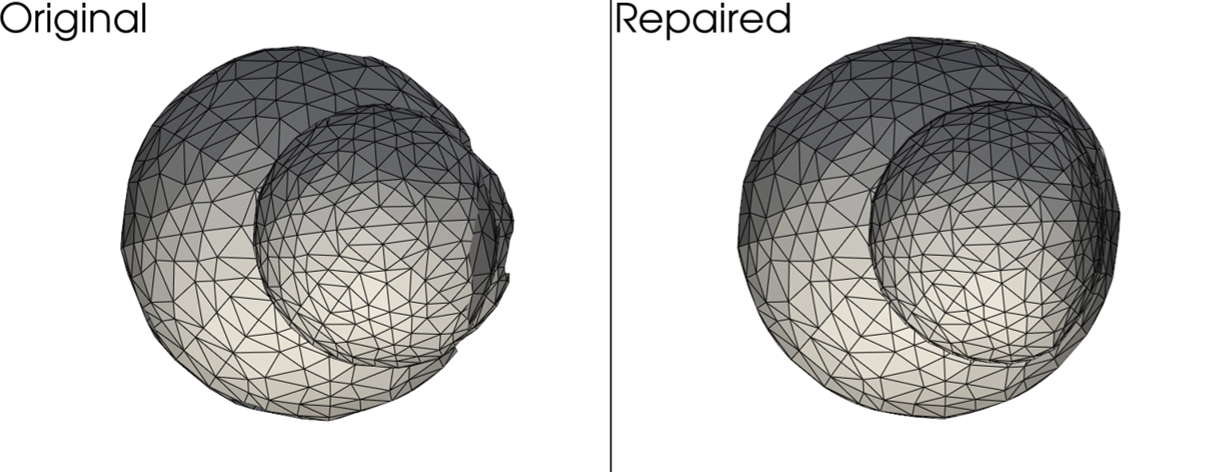
\includegraphics[ height=2.2cm]{../figures/new5.png}
    \caption{\textbf{Detaching enclosed meshes.} Original and repaired mesh for a test case with one sphere enclosed by another. The result is two distinct meshes without intersections.}
    \label{fig:sol2-2}
\end{figure}
\vspace{-1em}
\section{Conclusion}

% \TODO{DH: we can skip the summary here and just start with We evaluate XX and introduce YYY... so no history recap here to save space} Self-intersections in meshes have been studied for decades, and a large number of solutions and repair tools have been proposed. If one's sole objective is to eliminate intersections, in other words, reduce the count to zero, many existing methods--particularly those that subdivide problematic facets--would perform adequately. However, when mesh quality is equally crucial, these standard approaches may fall short. In such contexts, improving mesh quality becomes necessary, potentially through remeshing the affected regions where self-intersections were observed. Moreover, there are scenarios in which simple mesh repair is not sufficient. When it is important to distinguish between different submeshes during intersection resolution, detaching or controlled cutting may be required to preserve their structural meaning.
% The solutions implemented in this study are preliminary prototype designed to explore various methods to address these challenges. Future work will include enhancing its efficiency and robustness of the algorithm, validating it across more datasets, re-implementing it in C++ to improve performance. Ultimately, further research and mesh libraries development should also aim to provide ways that consider mesh quality while resolving self-intersections.

We evaluated several existing methods to merge neighboring meshes that intersect and introduced a new approach. Even when the repaired mesh was geometrically correct, the results were structurally and qualitatively different, hence the optimal method depends on the application, and quality metrics need to be carefully evaluated. Our method resulted in geometrically correct meshes of high quality. Furthermore, we proposed the first successful strategies for detaching intersecting meshes in cases where it is important to distinguish between different substructures. 
The solutions implemented in this study are preliminary prototypes. Future work will include enhancing their quality, efficiency and robustness, validating across more datasets. Further research and mesh library development should also aim to provide ways that improve mesh quality while resolving self-intersections.




%%
%% The next two lines define the bibliography style to be used, and
%% the bibliography file.
\bibliographystyle{ACM-Reference-Format}
\bibliography{template}


\end{document}
\endinput
%%
%% End of file `sample-sigconf-authordraft.tex'.
